% DO NOT COMPILE THIS FILE DIRECTLY!
% This is included by the other .tex files.

\begin{frame}[t,plain]
\titlepage
\end{frame}

\begin{frame}[t]{Topics for Today}
We will look at:

\begin{itemize}
\item Trans-dimensional MCMC
\item Nested Sampling
\end{itemize}

\end{frame}


\begin{frame}[t]{Trans-dimensional MCMC}
Trans-dimensional MCMC is useful when the model dimension is unknown. This
arises quite frequently in astrophysics.
\end{frame}


\begin{frame}[t]{Trans-dimensional examples}
Some examples from my own work: How many stars are in these images (and what are their positions and fluxes)?

\begin{center}
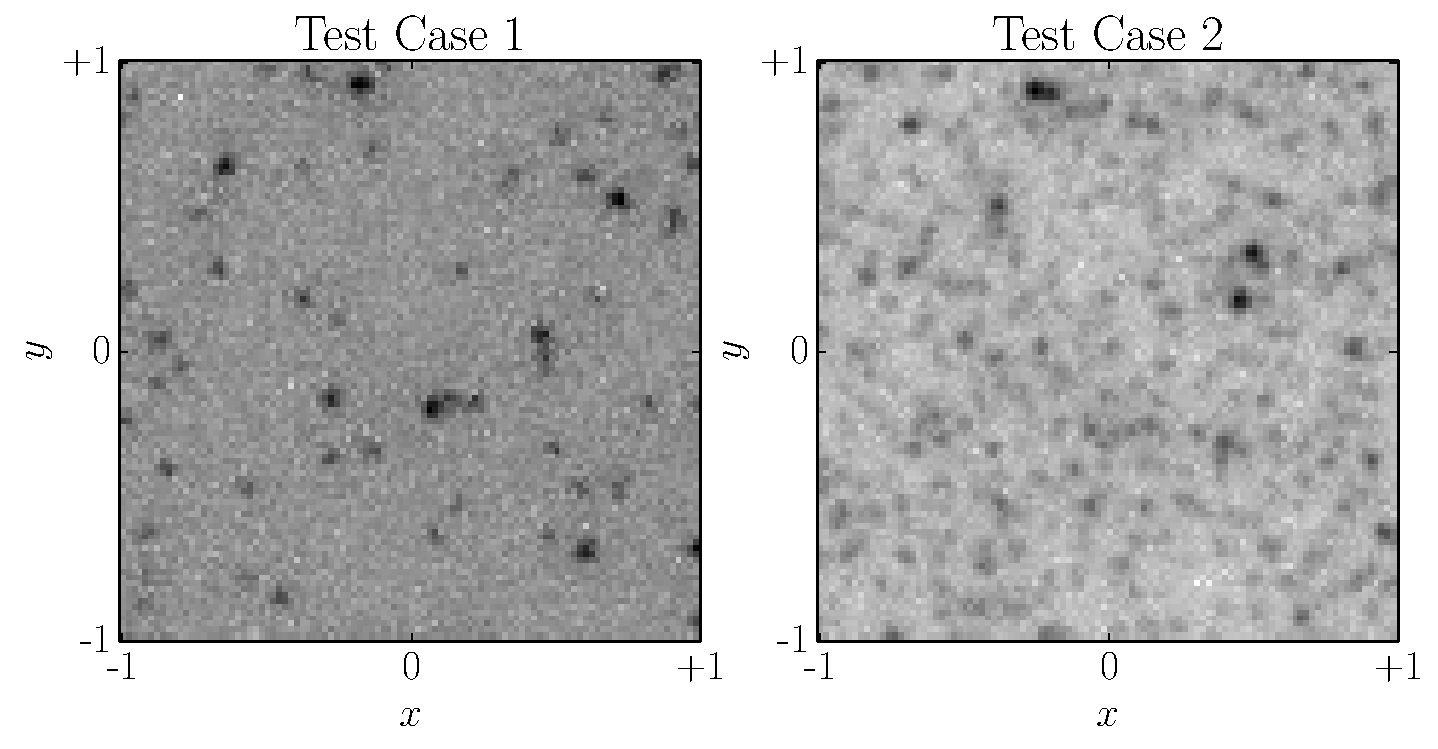
\includegraphics[scale=0.4]{starfield.pdf}
\end{center}

\end{frame}

\begin{frame}[t]{Trans-dimensional examples}
How many stars were there?

\begin{center}
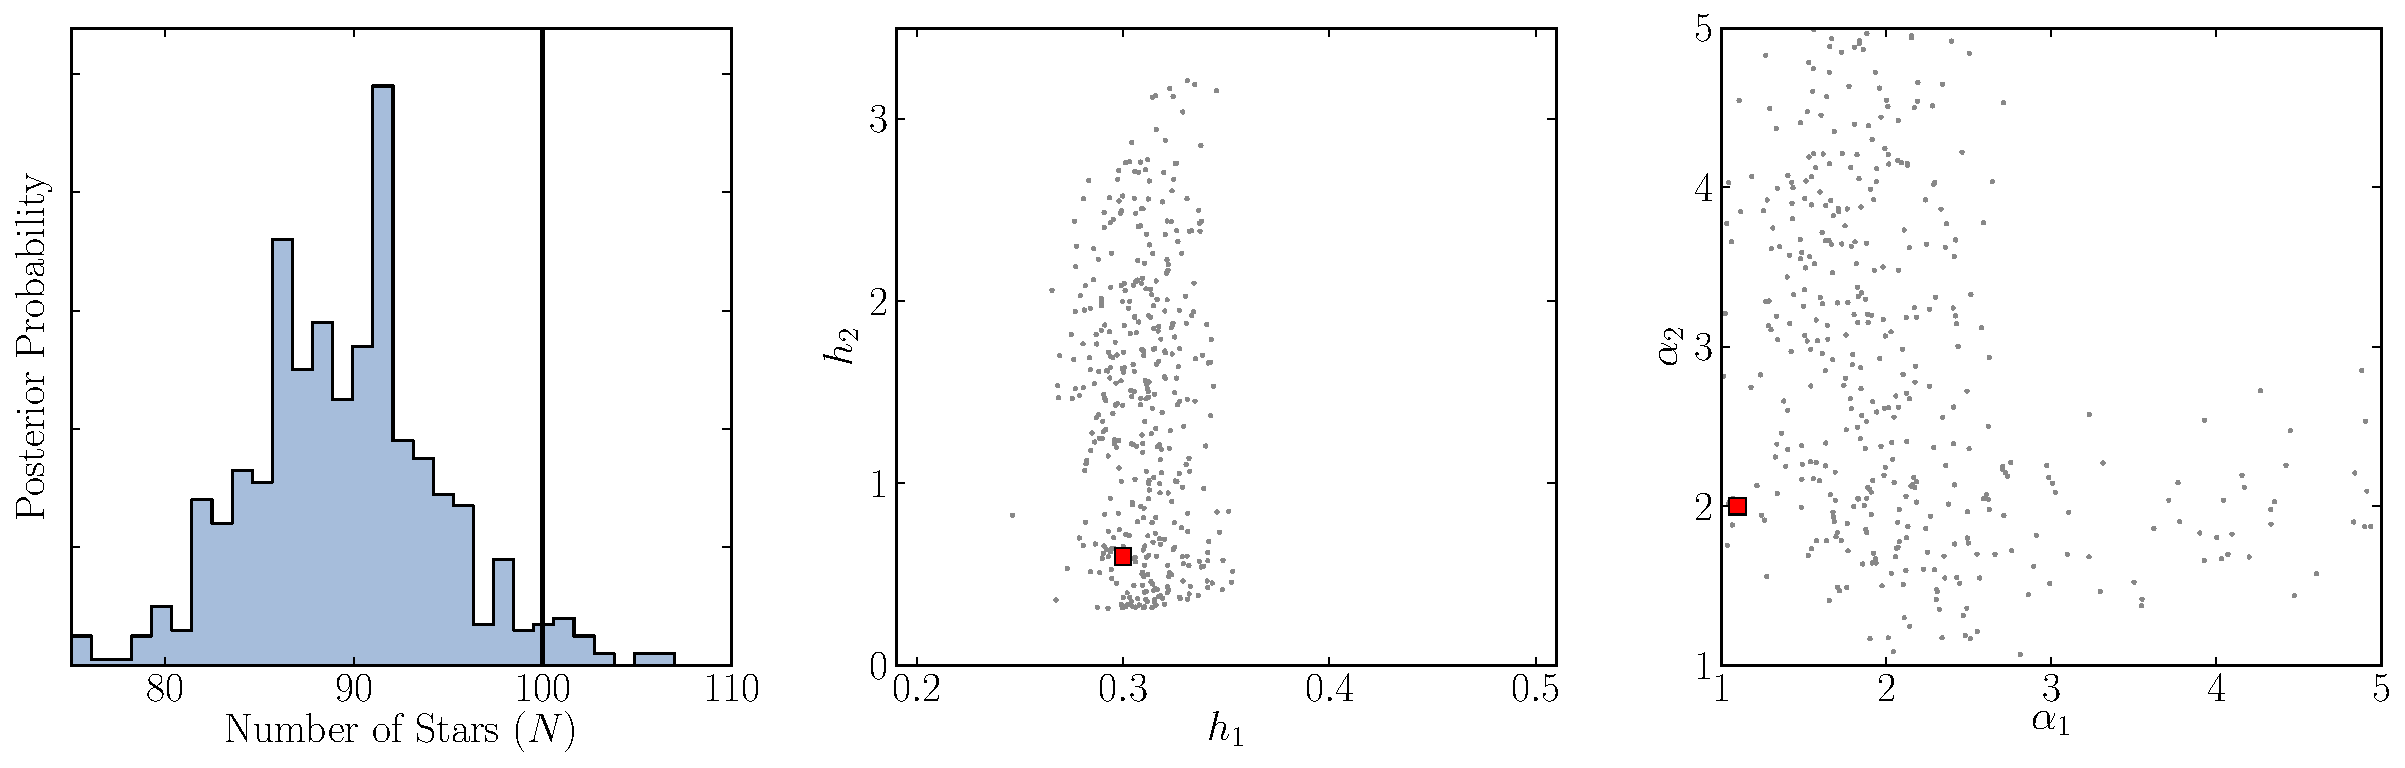
\includegraphics[scale=0.25]{inference1.pdf}
\end{center}

\end{frame}

\begin{frame}[t]{Trans-dimensional examples}
How many stars were there?
\begin{center}
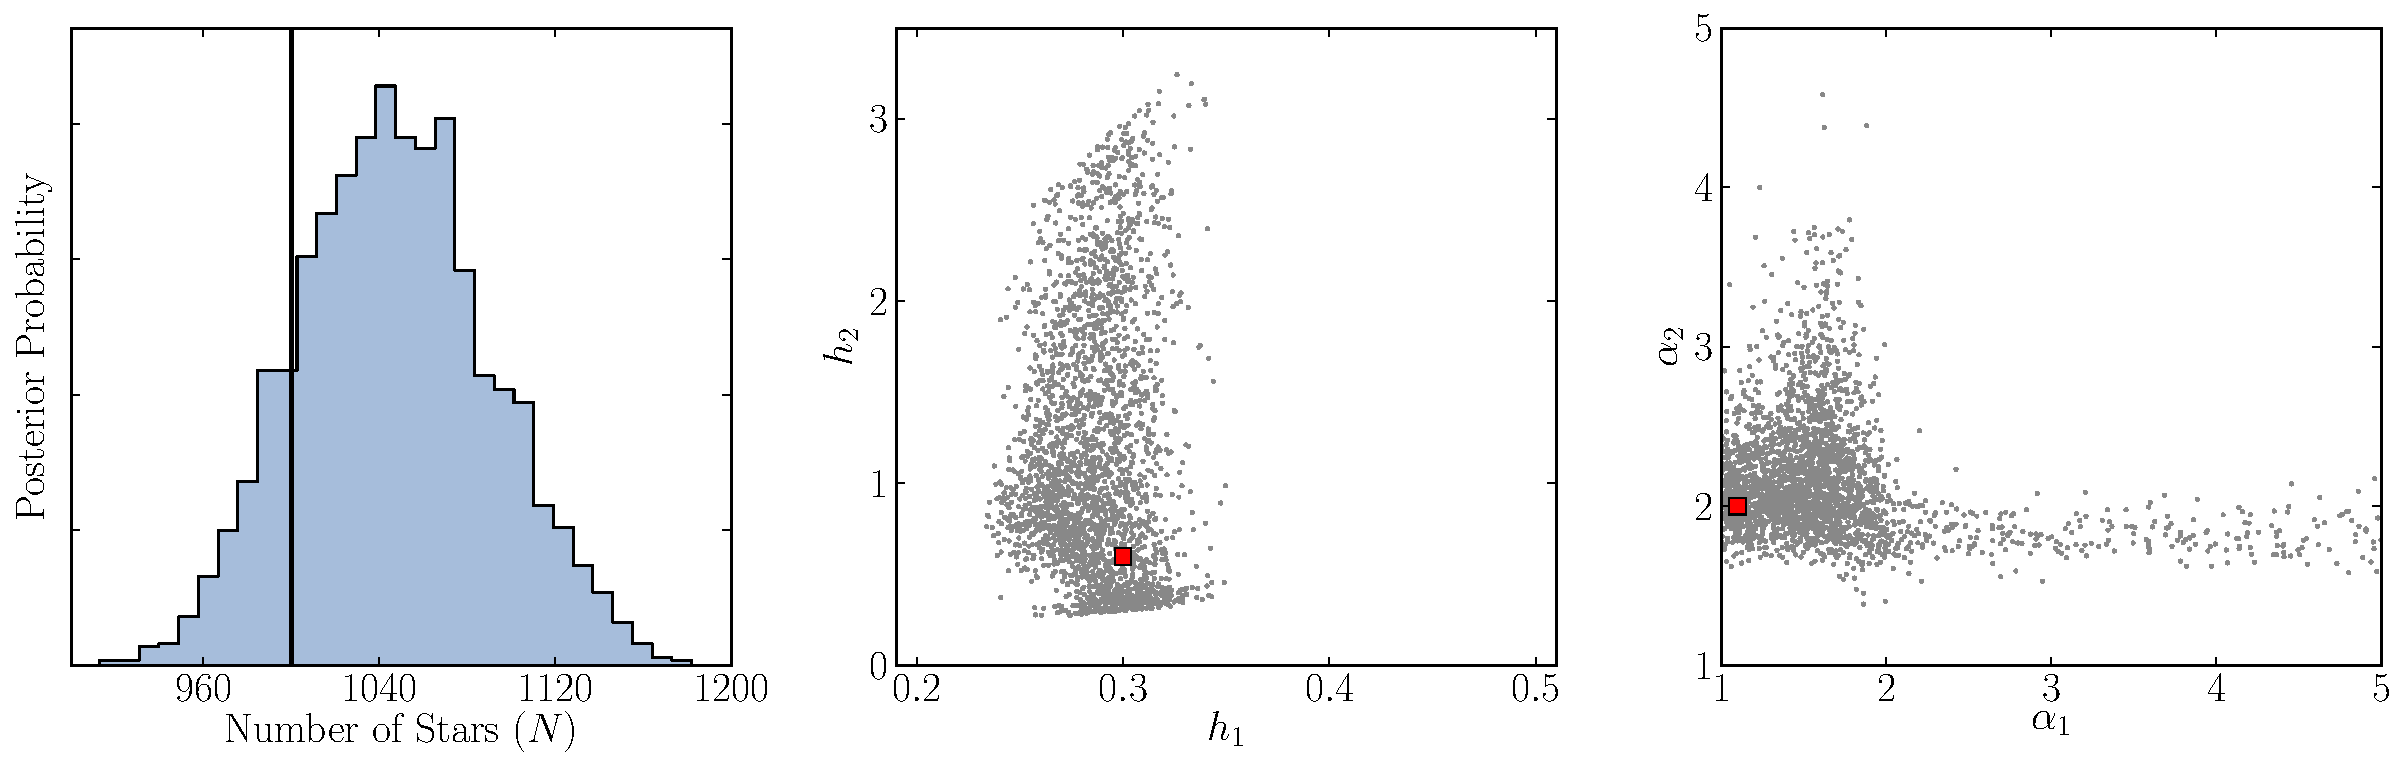
\includegraphics[scale=0.25]{inference2.pdf}
\end{center}

\end{frame}


\begin{frame}[t]{Birth and Death}
For problems of unknown dimensionality, the hypothesis space is the union
of several fixed-dimension hypothesis spaces. Can add {\bf birth and death}
proposals that try to increase or decrease the number of objects in the model.

\begin{center}
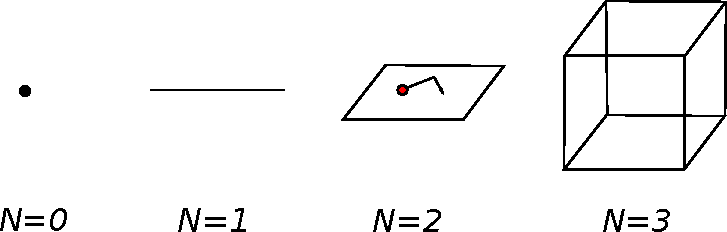
\includegraphics[scale=0.7]{drawing.pdf}
\end{center}

\end{frame}

\begin{frame}[t]{Asteroseismology Example}


\begin{center}
\includegraphics[scale=0.4]{Code/asteroseismology_data.pdf}
\end{center}

\end{frame}


\begin{frame}[t]{Asteroseismology Example}
Each of the peaks has a ``Lorentzian'' shape
(same as the Cauchy distribution!):
\begin{eqnarray}
m(x) &=& B + \sum_{i=1}^N \frac{A_i}
{\left[1 + \left(\frac{x - c_i}{w_i}\right)^2\right]} 
\end{eqnarray}

$A_i$ = amplitude of $i$th component\\
$c_i$ = center of $i$th component\\
$w_i$ = width of $ith$ component\\


\end{frame}

\begin{frame}[t]{Asteroseismology Example}
The sampling distribution/likelihood is

\begin{eqnarray*}
y_i \sim \textnormal{Exponential}(m(x_i; \theta)).
\end{eqnarray*}

i.e.
\begin{eqnarray*}
p(\{y_i\} | \theta) &=& \prod_{i=1}^n \frac{1}{m(x_i; \theta)}
\exp\left[-\frac{y_i}{m(x_i; \theta)}\right].
\end{eqnarray*}
\end{frame}



\begin{frame}[t]{Part II: Nested Sampling}
Nested Sampling is a Monte Carlo method (not necessarily MCMC) that was
introduced by John Skilling in 2004.

It is very popular in astrophysics and has some unique strengths.
\end{frame}


\begin{frame}[t]{Marginal Likelihood}
The {\bf marginal likelihood} is useful for ``model selection''. Consider
two models: $M_1$ with parameters $\theta_1$, $M_2$ with parameters $\theta_2$.
The marginal likelihoods are:
\begin{eqnarray*}
p(D | M_1) &=& \int p(\theta_1 | M_1) p(D | \theta_1, M_1) \, d\theta_1\\
p(D | M_2) &=& \int p(\theta_2 | M_2) p(D | \theta_2, M_2) \, d\theta_2
\end{eqnarray*}

These are the normalising constants of the posteriors, within each model.
\end{frame}



\begin{frame}[t]{Bayesian Model Selection}
If you have the marginal likelihoods, it's easy:

\begin{eqnarray*}
\frac{P(M_1 | D)}{P(M_2 | D)} &=& \frac{P(M_1)}{P(M_2)}
\times \frac{P(D | M_1)}{P(D | M_2)}.
\end{eqnarray*}
\end{frame}


\begin{frame}[t]{Challenging features}
\begin{center}
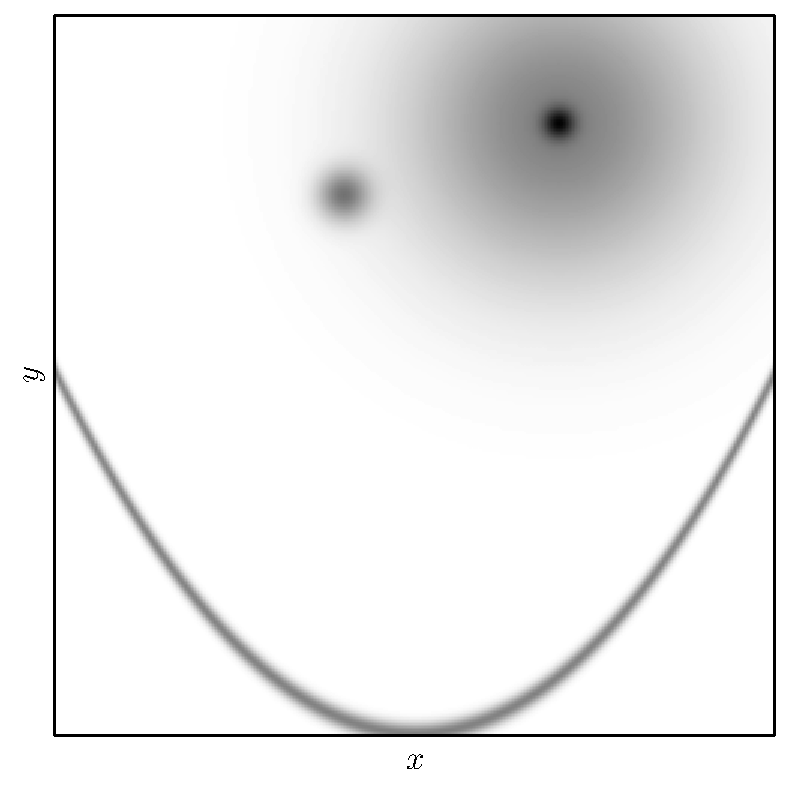
\includegraphics[scale=0.4]{challenges.pdf}
\end{center}
\end{frame}

\begin{frame}[t]{Nested Sampling}


\begin{figure}
\begin{center}
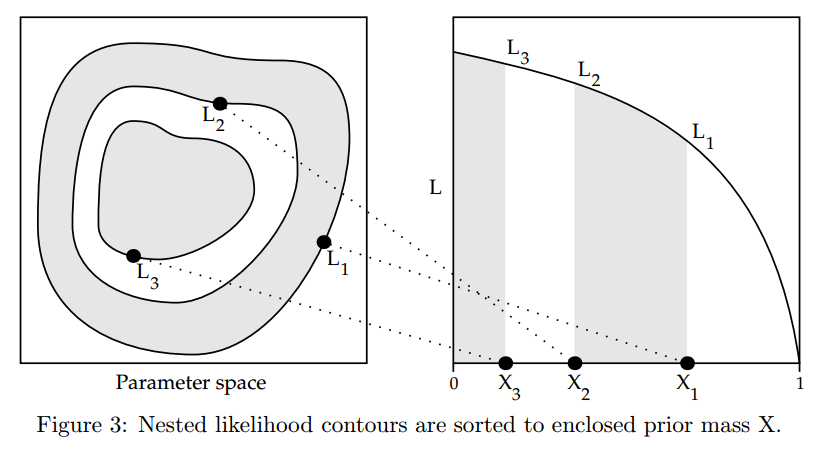
\includegraphics[scale=0.2]{ns.png}
\end{center}
\end{figure}

\end{frame}

